% \chapter{Life-Cycle Cost Analysis}
% \chapter{\texorpdfstring{\acrlong{lcca}}{全生命周期成本分析}}\label{chp:lcca}
\chapter[全生命周期成本分析]{\acrlong{lcca}}\label{chp:lcca}
% \section{Introduction}
\section{简介}
% This chapter introduces life-cycle cost analysis (LCCA) and its use in the decision making process for selecting optimum cost effective bridge systems, subsystems, and elements that can achieve long term service life. It includes general guidelines and best practices for application of LCCA, and outlines the steps in the process, along with a brief discussion of the economic principals involved. References to available models are made without recommending the use of a specific software or model.
本章介绍了\acrfull{lcca}及其在选择具有成本效益的最佳桥梁\gls*{system}、\gls*{subsystem}和可实现长期使用寿命的\gls*{element}的决策过程中的应用。它包括应用\acrlong{lcca}的一般指南和最佳实践,并概述了过程中的步骤,以及对所涉及的经济原则的简要讨论。对可用模型的引用并不推荐使用特定软件或模型。

% The use of LCCA, in lieu of purely initial construction cost evaluation, is essential in evaluating the long-term benefit of many strategies that can achieve extended service life (in excess of 100 years) yet require additional and sometimes considerable initial investment. LCCA can assist agencies with investment decisions by considering initial costs and relevant future costs associated with required inspection, maintenance, rehabilitation, and possible component replacement, including associated demolition, disposal, and user costs.

使用\acrlong*{lcca}代替纯粹的初始建设成本评估,对于评估许多可以实现延长使用寿命(超过 100 年)但需要额外且有时相当大的初始投资的策略的长期效益至关重要。 \acrlong*{lcca}可以通过考虑初始成本和与所需检查、维护、修复和可能的\gls*{component}更换相关的相关未来成本,包括相关的拆除、处置和用户成本,进而帮助机构做出投资决策。

% In its broadest form, LCCA can be used in the evaluation of alternative bridge systems. In its more simplified forms, it aids in evaluating alternatives for bridge components such as decks, superstructures, substructures, or more specialized bridge element applications, such as comparing alternatives for deck joints or bearings.

在其最广泛的形式中,\acrlong*{lcca}可用于评估桥梁系统方案。在其更简化的形式中,它有助于评估桥梁\gls*{component}的备选方案,例如桥面系、上部结构、下部结构或更专业的桥梁\gls*{element}应用,例如比较桥面连续或支座的备选方案。

% This chapter is intended to provide only a brief discussion of the benefits, principles and methodologies involved in LCCA. Additional detail on this entire process and its application is provided in the attached references, primarily in the Life-Cycle Cost Analysis Primer (FHWA 2002), and in NCHRP Report 483, Bridge Life-Cycle Cost Analysis (Hawk 2003).

本章旨在仅简要讨论\acrlong*{lcca}中涉及的好处、原则和方法。附加参考资料中提供了有关整个过程及其应用的更多详细信息,主要是 \bkn*{Life-Cycle Cost Analysis Primer} \cite{fhwa2002l} 和 \gls{nchrp} 报告 483,\bkn*{Bridge Life-Cycle Cost Analysis} \cite{hawk2003b}。

% \section{LCCA Defined}
% \section{\texorpdfstring{\acrlong{lcca}}{全生命周期成本分析}的定义}
\section[全生命周期成本分析的定义]{\acrlong*{lcca}的定义}
% LCCA is an analysis methodology that assists in comparing and choosing alternative strategies for achieving long-term service life for bridge systems, subsystems or elements. It considers not only the initial construction cost, but also all of the costs that are expected to occur over the entire service life of the bridge, typically maintenance, major rehabilitation, and component or element replacement, including relevant demolition and disposal costs, and user costs. Economic methods are used to convert anticipated future costs to present dollar values so that lifetime costs of various alternatives can be directly compared.
\acrlong*{lcca}是一种分析方法,有助于比较和选择备选策略,以实现桥梁\gls*{system}、\gls*{subsystem}或\gls*{element}的长期\gls*{servicelife}。它不仅考虑初始建设成本,还考虑桥梁整个使用寿命期间预期发生的所有成本,通常是维护、大修和\gls*{component}或\gls*{element}更换,包括相关的拆除和处置成本,以及用户费用。经济方法用于将预期的未来成本转换为当前的美元价值,以便可以直接比较各种替代方案的生命周期成本。

% \subsection{Steps in LCCA}
\subsection{\texorpdfstring{\acrlong*{lcca}}{全生命周期成本分析}的步骤}
% There are five basic steps in the LCCA process, which are described in the following sections (FHWA 2002).
在\acrlong{lcca}过程中有五个基本步骤,将在以下部分进行描述 \cite{fhwa2002l}。
% \paragraph*{Step 1. Establish Design Alternatives}
\paragraph*{步骤 1. 建立设计备选方案}
% This step involves establishing the elements of initial design and identifying the associated activities that will be required throughout its service life for maintenance, rehabilitation, or element replacement within a system or subsystem—for each alternative being considered.
此步骤涉及建立初始设计的要素,并对于正在考虑的每个备选方案,确定在\gls*{system}或\gls*{subsystem}内维护、修复或\gls*{element}更换的整个使用寿命期间所需的相关活动。

% \paragraph*{Step 2. Determine Activity Timing}
\paragraph*{步骤 2. 确定活动时间}
% The timing of associated activities throughout the period of comparison must be determined as part of the identification process. Estimating when and how often certain activities must be performed is important in making realistic comparisons. This process might involve identifying certain required maintenance on a yearly basis, or certain levels of potential rehabilitation due to expected wear after a specified period of time, or when individual components or elements such as decks or bearings may have to be replaced. Agency data is important in establishing when various levels of maintenance, rehabilitation or replacement may be required. In the absence of data, expert opinion can be used.
整个比较期间相关活动的时间安排必须作为识别过程的一部分来确定。 估计某些活动必须执行的时间和频率对于进行现实比较很重要。这个过程可能涉及确定每年需要进行的某些维护,或由于指定时间段后的预期磨损而导致的某些潜在修复水平,或者可能必须更换单个\gls*{component}或\gls*{element}(例如桥面板或支座)的时间。 机构数据对于确定何时可能需要进行各种级别的维护、修复或更换很重要。在没有数据的情况下,可以使用专家意见。

% \paragraph*{Step 3. Estimate Costs}
\paragraph*{步骤 3. 估算成本}
% This step involves estimating the initial construction cost associated with each design alternative and the costs associated with the various identified future maintenance, rehabilitation, and replacement activities. Costs are computed on the basis of current cost data. It is recommended as a best practice that costs include both agency costs and user costs. This is discussed further in \cref{subsec:lcca-cost-types}.
此步骤涉及估算与每个设计备选方案相关的初始施工成本以及与各种已确定的未来维护、修复和更换活动相关的成本。成本是根据当前成本数据计算的。作为最佳实践,建议成本包括代理成本和用户成本。这将在\cref{subsec:lcca-cost-types}中进一步讨论。

% \paragraph*{Step 4. Compute Life-Cycle Costs}
\paragraph*{步骤 4. 计算\acrlong*{lcc}}
% This step involves computing the \acrfull{pv} of all costs identified for a given alternative. The concepts of \acrshort{pv} are further discussed in \cref{subsec:npv}. As part of this computational process, there are two approaches, either deterministic or stochastic (probabilistic), that address the variability and uncertainty associated with input factors. The deterministic approach (most used) uses fixed discreet values while the stochastic approach defines input   variables by a probability distribution. These computational approaches are further discussed in \cref{subsec:computational-approaches}.
此步骤涉及计算给定备选方案确定的所有成本的\acrfull{pv}。 \acrshort{pv} 的概念在\cref{subsec:npv}中进一步讨论。作为此计算过程的一部分,有两种方法,即确定性方法或随机性(概率)方法,用于解决与输入因素相关的可变性和不确定性。确定性方法(最常用)使用固定离散值,而随机方法通过概率分布定义输入变量。这些计算方法在\cref{subsec:computational-approaches}中进一步讨论。

% \paragraph*{Step 5. Analyze Results}
\paragraph*{步骤 5. 分析结果}
% This step involves comparing the initial and life-cycle costs associated with the various alternatives and determining the optimal cost-effective solution. If the alternatives provide different levels of service, then the alternatives that provide the best overall long-term benefit can also be compared.
此步骤涉及比较与各种备选方案相关的初始成本和\acrlong*{lcc},并确定最佳的成本效益解决方案。如果备选方案提供不同级别的服务,那么也可以比较提供最佳总体长期利益的备选方案。

% \subsection{LCCA Cost Types}
\subsection{\texorpdfstring{\acrlong*{lcca}}{全生命周期成本分析}成本类型}
\label{subsec:lcca-cost-types}
% \subsubsection{Agency Costs}
\subsubsection{代理成本}
% These costs include all the costs born by the agency or owner of the bridge, including design, initial construction, inspection, maintenance, rehabilitation, and element replacement, and have been the primary elements for consideration in \arclong{lcca}. Some costs such as initial construction, rehabilitation, and replacement are more easily estimated based on current industry cost data. Other costs, such as maintenance, are more difficult and rely on the existence and accuracy of agency historical cost data. In the absence of this data, expert opinion can be used.
这些成本包括桥梁的主管机构或业主承担的所有成本,包括设计、初始施工、检查、维护、修复和\gls*{element}更换,并且已成为\acrlong*{lcca}考虑的主要要素。根据当前的行业成本数据,更容易估算初始建设、修复和更换等一些成本。其他成本,如维护,难度更大,依赖于机构历史成本数据的存在和准确性。在没有此数据的情况下,可以使用专家意见。

% \subsubsection{User Costs}
\subsubsection{用户成本}\label{subsubsec:user-costs}
% These costs are primarily associated with reduced traffic capacity in work zones, and involve costs to the users because of delays, vehicle operating costs, and accidents. Estimating these costs may be the greatest challenge to LCCA implementation. Many agencies have been reluctant to incorporate user costs in LCCA because of difficulty and uncertainty in assigning value to user delay time, or because user costs are not factored into agency budgets. These issues have led many agencies to give lesser credence to user costs in evaluating overall lowest cost solutions; however, minimizing user impacts and associated costs is a major concern today, especially with implementation of \acrfull*{abc}. A recent pooled-fund study led by the Oregon \acrfull{dot} \cite{doolen2011a} developed a set of decision making tools to determine if \acrshort*{abc} techniques are more effective that traditional construction for a given bridge replacement or rehabilitation project. These tools incorporate quantified user costs as part of a life-cycle cost analysis evaluation.
这些成本主要与\gls*{workzone}交通能力降低有关,并且涉及因延误、车辆运营成本和事故而给用户带来的成本。估算这些成本可能是\acrlong*{lcca}实施的最大挑战。许多机构一直不愿意将用户成本纳入\acrlong*{lcca},因为在为用户延迟时间分配价值时存在困难和不确定性,或者因为用户成本未计入机构预算。这些问题导致许多机构在评估总体成本最低的解决方案时不太相信用户成本。然而,最小化用户影响和相关成本是当今的一个主要问题,尤其是在实施\gls{abc}时。 最近由俄勒冈州\acrshort*{dot} \cite{doolen2011a} 领导的一项联合基金研究开发了一套决策工具,以确定 \gls{abc} 技术是否比传统施工更有效地更换或修复给定的桥梁项目。 这些工具将量化的用户成本作为生命周期成本分析评估的一部分。

% User costs can play an important factor in evaluating various options for long-term service life. {subsec:estimate-user-costs} further discusses the approach for estimating user costs based on traffic volumes and user delays.
用户成本是评估长期使用寿命的各种选择的重要因素。 \cref{subsec:estimate-user-costs}进一步讨论了根据流量和用户延迟估算用户成本的方法。

% \subsubsection{Vulnerability Costs}
\subsubsection{漏洞成本}
% These costs are associated with extraordinary circumstances and risks, such as overload, collision, blast, fire, floods, scour, or earthquake, and typically would not be included in LCCA for comparison of service life strategies. They are useful, however, in evaluating vulnerability of existing bridges that might have high probability for one or more of these extraordinary events.
这些成本与特殊情况和风险有关,例如超载、碰撞、爆炸、火灾、洪水、冲刷或地震,通常不会包含在\acrlong*{lcca}中以比较使用寿命策略。然而,它们有助于评估现有桥梁的脆弱性,这些桥梁极有可能发生这些异常事件中的一个或多个。

% \subsection{LCCA Versus Benefit-Cost Analysis (BCA)}
\subsection{\texorpdfstring{\acrlong*{lcca}}{全生命周期成本分析}与\texorpdfstring{\acrfull*{bca}}{效益成本分析}的比较}
% \subsection[全生命周期成本分析与效益成本分析的比较]{\acrlong*{LCCA}与\acrfull*{BCA}的比较}

% \acrlong*{lcca} is a subset of benefit cost analysis, which compares benefits as well as costs in selecting optimal alternatives. \acrlong*{bca} is useful in comparing alternatives that do not achieve the same level of service or benefit. For example, \acrlong*{bca} can be useful in comparing bridge replacement options that provide either three or four lanes of traffic with corresponding different levels of service. Clearly there are both cost and benefit variations between each option. \acrlong*{lcca} is typically considered alone for service life evaluation of various alternatives that can ultimately provide the same level of service.
\acrlong*{lcca} 是\acrfull*{bca}的一个子集,它比较了选择最优方案时的收益和成本。 \acrlong*{bca}在比较未达到相同服务水平或收益的备选方案时很有用。例如,\acrlong*{bca}可用于比较提供三车道或四车道交通的桥梁替换选项以及相应的不同服务级别。 显然,每个选项之间都存在成本和收益差异。\acrlong*{lcca}通常被单独考虑用于评估最终可以提供相同服务水平的各种替代方案的使用寿命。

% \section{Elements of LCCA}
\section[全生命周期成本分析的要素]{\acrlong*{lcca}的要素}
% This section discusses methodologies for determining net present value and discount rates. It further discusses other elements considered in LCCA such as activity timing and service life, user costs, computational approaches, and analysis tools.
本节讨论确定\acrlong*{npv}和贴现率的方法。 它进一步讨论了\acrlong*{lcca}中考虑的其他要素,例如活动时间和使用寿命、用户成本、计算方法和分析工具。

% \subsection{Net Present Value (NPV)}
\subsection{\texorpdfstring{\acrlong*{npv}}{净现值(NPV)}}
\label{subsec:npv}
% The net present value concept in LCCA is an economic method for combining initial costs and present dollar values of future expected costs so that lifetime costs for various alternatives can be directly compared. Dollars spent at different times within a structures life have different present values, so the projected activity costs for an alternative cannot simply be added together to calculate the total life cycle cost for that alternative. A dollar today is worth more than a dollar five years from now, even if there is no inflation because today's dollar can be used productively in the ensuing five years, yielding a value greater than the initial dollar. Future benefits and costs are discounted to reflect this fact.
\acrlong*{lcca}中的\acrlong*{npv}概念是一种将初始成本与未来预期成本的现值相结合的经济方法,以便可以直接比较各种备选方案的生命周期成本。在结构寿命的不同时间花费的美元具有不同的\acrlong*{pv},因此不能简单地将替代方案的预计活动成本加在一起来计算该替代方案的总生命周期成本。即使没有通货膨胀,今天的一美元也比五年后的一美元值钱,因为今天的美元可以在随后的五年中得到有效利用,产生的价值高于最初的美元。 未来的收益和成本被贴现以反映这一事实。

% The purpose of discounting is to put all present and future costs into a common metric, their net present value.
贴现的目的是将所有现在和未来的成本放入一个共同的指标中,即它们的净现值。

% The formula to convert the sum of the initial cost and the present value of future repair and renewal costs into net present value is given by \cref{eq:net-present-value}.
将初始成本与未来维修和更新成本的现值之和转换为净现值的公式由 \cref{eq:net-present-value} 给出。
\begin{equation}
  \label{eq:net-present-value}
  \mathrm{NPV} =\text{initial cost} + \sum\limits_{k=1}^N \text{rehab cost}_k \left[ \frac{1}{(1+r)^{n_k}}\right]
\end{equation}
\begin{EqDesc}{n_k}
  \item [r] 实际贴现率;
  \item [k] 未来进行的修复活动的序号;
  \item [N] 修复活动总数;
  \item [n_k] 未来成本发生的那一年。
\end{EqDesc}

\medskip
% The term $\left[ \frac{1}{(1+r)^{n_k}}\right]$ is called the discount factor.
$\left[ \frac{1}{(1+r)^{n_k}}\right]$ 这一项称为贴现因子。

\medskip
% Input factors in computing NPV are the initial cost (usually the cost of planning, design and construction of a new structure), the cost and timing of rehabilitation activities, and the real discount rate.
计算\acrlong*{npv}的输入要素是初始成本(通常是新结构的规划、设计和建造成本)、修复活动的成本和时间以及实际贴现率。

% Discounting is a method of considering the opportunity cost of money as it applies to current versus future funds. It can be thought of in terms of the alternative economic return that could be gained on funds such as earning interest. The computed potential amount of interest is based on what is referred to as the discount rate, which is generally described as having three components:
贴现是一种考虑货币机会成本的方法,因为它适用于当前与未来的资金。可以从诸如赚取利息的资金中获得的替代经济回报的角度来考虑。计算出的潜在利息金额基于所谓的贴现率,贴现率通常被描述为具有三个组成部分:

% \begin{enumerate}
%   \item The real opportunity cost of capital to account for productive value of funds;
%   \item The premium to account for financial risk (i.e. that the loan will not be repaid); and
%   \item The anticipated rate of inflation.
% \end{enumerate}
\begin{enumerate}
  \item 资金的实际机会成本,用于说明资金的生产价值;
  \item 考虑财务风险的溢价(即贷款不会被偿还);
  \item 预期的通货膨胀率。
\end{enumerate}

% Life-cycle analyses typically ignore inflation because the prediction of future prices introduces unnecessary uncertainty into the analysis. Therefore, discount rates are typically based on interest rates for government borrowing, which have little risk, with the inflation component removed, yielding the "real" interest rate. This rate is typically calculated by subtracting the rate of inflation (consumer price index) from the interest rate of an investment such as a 10-year U.S. Treasury bill. For example, if the interest on a 10-year Treasury bill is 5.5\% and the inflation rate is 3\%, then the discount rate would be 2.5\%.
\acrlong*{lcca}通常会忽略通货膨胀,因为对未来价格的预测会在分析中引入不必要的不确定性。因此,贴现率通常基于风险很小的政府借款的利率,在去除了通货膨胀因素后产生“实际”利率。该利率通常是通过从 10 年期美国国库券等投资利率中减去通货膨胀率(消费者价格指数)计算得出的。例如,如果 10 年期国库券的利率为 5.5\%,通货膨胀率为 3\%,则贴现率为 2.5\%。

% OMB Circular No. A94 (OMB 1992) provides general guidance for conducting cost-effectiveness analyses, and provides specific guidance on the discount rates to be used in evaluating programs whose benefits and costs are distributed over time. It provides standard criterion for deciding whether programs can be justified on economic principles, and the OMB publishes real interest rates for net present value analyses on its website.
\acrfull*{omb} 通告第 A94 号 \cite{omb1992} 为进行成本效益分析提供了一般指导,并为用于评估收益和成本随时间分配的计划的贴现率提供了具体指导。它为决定计划是否可以根据经济原则合理提供了标准标准,\acrshort*{omb} 在其网站上公布了净现值分析的实际利率。

% The discount rate can have a significant impact on the analysis, as can be seen in \cref{fig:effect- discount-rates}. A low discount rate favors projects with long-term benefits and near-term costs. When evaluating alternative projects, a sensitivity analysis using a range of discount rates can be used to determine the importance or impact of the discount rate in the relative project performance. Even with a low discount rate, values far in the future have a relatively low present value.
贴现率会对分析产生重大影响,如 \cref{fig:effect-discount-rates} 所示。低贴现率有利于具有长期利益和近期成本的项目。在评估备选项目时,使用一系列贴现率的敏感性分析可用于确定贴现率在相关项目绩效中的重要性或影响。 即使贴现率很低,未来的价值也具有相对较低的现值。

\begin{figure}
  % \includegraphics[width=\linewidth]{graphic-file}
  % \caption{Effect of discount rates on present value}
  \caption{贴现率对现值的影响}
  \label{fig:effect-discount-rates}
\end{figure}

% \subsection{Activity Timing, Service Life, and Life Cycle}
\subsection{活动时序、\glsentrytext{servicelife}和生命周期}

% \subsubsection{Deterioration Models}
\subsubsection{\gls*{deterioration}模型}
% Deterioration models describe the relationship between the condition of the bridge (or its element) and time, showing how the bridge deteriorates. It assumes that no replacements or major repairs are made, but it usually implies that scheduled maintenance actions are performed as planned. The basic model applies either to a bridge as a whole, or to any of its elements (e.g., deck, substructure, bearings, columns). The shape of a deterioration curve depends on the type of the element and the definitions of condition states.
\gls*{deterioration}模型描述了桥梁(或其\gls*{element})的状况与时间之间的关系,显示了桥梁如何\gls*{deterioration}。它假设没有进行任何更换或大修,但通常意味着按计划执行了定期维护操作。基本模型既适用于整个桥梁,也适用于其任何\gls*{element}(例如,桥面系、下部结构、支座、柱子)。 \gls*{deterioration}曲线的形状取决于\gls*{element}的类型和条件状态的定义。

% An example of a deterioration curve is presented in \cref{fig:bridge-deterioration-curve}. If the bridge is placed in service at period $T_0$, its condition gradually declines, and the deterioration curve represents its condition over time. Initially the condition is good, but after a period of wear and aging, it eventually (at time $T_\text{f}$) reaches an unacceptably low condition $C_\text{f}$. The time period between $T_0$ and $T_\text{f}$ is called the service life (SL) of the bridge.
\cref{fig:brg-deterioration-curve} 中给出了\gls*{deterioration}曲线的示例。 如果桥梁在 $T_0$ 期间投入使用,其状况会逐渐下降,\gls*{deterioration}曲线表示其状况随时间的推移。 最初状态良好,但经过一段时间的磨损和老化后,它最终($T_\text{f}$ 时刻)达到不可接受的低状态 $C_\text{f}$。 $T_0$ 和 $T_\text{f}$ 之间的时间段称为桥梁的\acrfull*{sl}。

\begin{figure}
  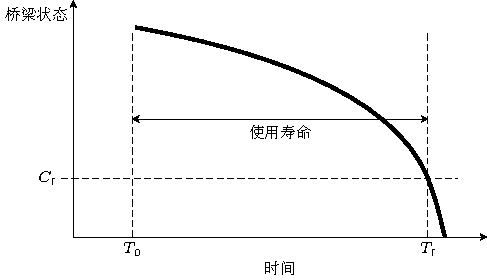
\includegraphics{bridge-deterioration-curve.pdf}
  \caption{Bridge deterioration curve}\label{fig:brg-deterioration-curve}
\end{figure}

% In practice however, realistic deterioration models that are based on actual physical and chemical deterioration processes are generally not available to accurately predict service life. The most acceptable deterioration model is in the form of the solution to Fick's second law, used to predict the rate of chloride ingress through concrete cover. This model, including its limitations, is described in \cref{chp:corrosion-of-steel-rc-bridge} of the Guide. It is expected that with time additional deterioration models will become available and will greatly enhance  uantification of the service life of bridge elements, components, subsystems or systems.
然而在实践中,基于实际物理和化学\gls*{deterioration}过程的现实\acrlong*{deterioration}模型通常无法准确预测使用寿命。 最可接受的\gls*{deterioration}模型采用菲克第二定律的解形式,用于预测氯离子通过混凝土保护层的侵入率。该模型及其局限性在\bkn{指南}的\cref{chp:corrosion-of-steel-rc-bridge}中进行了描述。 预计随着时间的推移,附加的\gls*{deterioration}模型将变得可用,并将大大提高桥梁\gls*{element}、\gls*{component}、\gls*{subsystem}或\gls*{system}\gls*{servicelife}的量化。

% Developing deterioration models is a data-intensive procedure and is complicated by the lack of knowledge of the underlying processes that foster deterioration as well as by data availability. In lieu of deterioration models based on actual physical and chemical deterioration processes, other approximate methods must be used. Bridge management software programs such as Pontis and BRIDGIT, which are used in nearly all 50 states, have deterioration models contained within them that are typically based on expert opinion and analysis of available historical data.
开发\gls*{deterioration}模型是一个数据密集型过程,并且由于缺乏对促进\gls*{deterioration}的基础过程的了解以及数据可用性而变得复杂。 代替基于实际物理和化学\gls*{deterioration}过程的\gls*{deterioration}模型,必须使用其他近似方法。 \pontis 和 BRIDGIT 等几乎所有 50 个州都在使用的桥梁管理软件程序中包含\gls*{deterioration}模型,这些模型通常基于专家意见和对可用历史数据的分析。

% Recent studies by the New York State DOT (Agrawal and Kawaguchi 2009) and the Florida DOT (Sobanjo 2011) have further attempted to develop bridge element deterioration models based on state DOT bridge inspection databases along with expert opinion. The New York State DOT study applied computerized statistical methods to develop deterioration curves using inspection data going back to 1981. The study included the influence of various factors such as average daily truck traffic (ADTT) and climate, among others.
纽约州\acrlong*{dot} \cite{agrawal2009b} 和佛罗里达州\acrlong*{dot} \cite{sobanjo2011d} 最近的研究进一步尝试开发基于州\acrlong*{dot}桥梁检查数据库以及专家意见的桥梁\gls*{element}\gls*{deterioration}模型。 纽约州\acrlong*{dot}研究采用计算机化统计方法,利用可追溯至 1981 年的检查数据绘制\gls*{deterioration}曲线。该研究包括各种因素的影响,例如\acrfull*{adtt}和气候等。

% The New York State DOT study further implemented a stochastic approach to account for the uncertainty and randomness of factors affecting the deterioration process. In the stochastic approach, the ratings of bridge elements (reflective of their condition at a particular time) and the durations that elements will stay at a particular rating were assumed to be random variables and were modeled by probability distributions. The study developed and compared deterioration curves using both Markov chain and Weibull-distribution based stochastic models. Markov chain is the most commonly used model for developing deterioration rates for infrastructure facilities, and is used in advanced bridge management systems such as Pontis and BRIDGIT. It models the deterioration process by considering the probability of transition from one condition state to another in a discrete time, and accounts for the current element condition in predicting the future condition. A Weibull-based model considers the probability of how long a bridge element will remain at a particular state, and also considers past conditions. The New York State DOT study found that the Weibul-based models generally provided the best overall fit with historical bridge inspection data.
纽约州\acrlong*{dot}研究进一步采用随机方法来解释影响\gls*{deterioration}过程的因素的不确定性和随机性。 在随机方法中,桥梁\gls*{element}的评级(反映它们在特定时间的状况)和\gls*{element}将保持在特定评级的持续时间被假定为随机变量,并通过概率分布建模。该研究使用基于马尔可夫链和韦伯分布的随机模型开发并比较了\gls*{deterioration}曲线。 马尔可夫链是开发基础设施退化率最常用的模型,用于先进的桥梁管理系统,如 \pontis 和 BRIDGIT。 它通过考虑在离散时间内从一种条件状态转换到另一种条件状态的概率来模拟\gls*{deterioration}过程,并在预测未来条件时考虑当前\gls*{element}条件。 基于韦伯分布的模型考虑了桥梁\gls*{element}将保持在特定状态多长时间的概率,并且还考虑了过去的条件。 纽约州\acrlong*{dot}研究发现,基于韦伯分布的模型通常提供与历史桥梁检查数据的最佳整体拟合。

% It should be noted that methods that use historical data to develop long term bridge element deterioration models have certain limitations. Aside from not considering the actual physical deterioration process, older historical data does not consider more recent improvements in construction materials or methods, which can greatly affect future service life. Further, there is some uncertainty about extrapolating the data beyond the duration for which the data was collected.
应该注意的是,使用历史数据开发长期桥梁\gls*{element}\gls*{deterioration}模型的方法有一定的局限性。除了不考虑实际的物理\gls*{deterioration}过程外,较旧的历史数据不考虑最近对建筑材料或方法的改进,这会极大地影响未来的\gls*{servicelife}。此外,在收集数据的持续时间之外推断数据存在一些不确定性。

% \subsubsection{Expenditure Stream}
\subsubsection{支出流}
% As shown on \cref{fig:bridge-condition-life-cycle}, a bridge will deteriorate over the period of its service life if left unattended. However, in most cases a bridge is not left to follow the basic deterioration path and reach an unacceptable condition without interruption. The agency responsible for the bridge will, from time to time, undertake repairs, rehabilitations, and renewals that return conditions to higher levels and extend its service life.
如\cref{fig:bridge-condition-life-cycle} 所示,如果无人看管,桥梁将在其使用寿命期间恶化。然而,在大多数情况下,桥梁不会沿着基本的退化路径发展并在不中断的情况下达到不可接受的状态。负责桥梁的机构将不时进行维修、修复和更新,使条件恢复到更高水平并延长其使用寿命。

\begin{figure}
  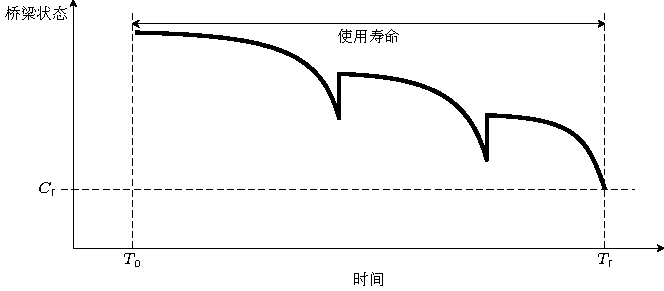
\includegraphics{condition-life-cycle.pdf}
  % \caption{Bridge condition life cycle}
  \caption{桥梁状况生命周期}
  \label{fig:bridge-condition-life-cycle}
\end{figure}

% The sequence of events and actions that determine the bridge condition throughout its life cycle is called Life Cycle Activity Profile. Actions are usually associated with expenditures that have to be incurred when repair, rehabilitation, and renewal activities are taking place. These expenditures may be plotted on a separate diagram that represents the stream of expenditures associated with construction and repair activities. Such a diagram is sometimes called a cash flow diagram. An example of such diagram is shown on \cref{fig:cash-flow-diagram}.
在整个生命周期中决定桥梁状况的事件和行动的顺序称为生命周期活动概况。行动通常与进行维修、修复和更新活动时必须发生的支出相关。这些支出可以绘制在一个单独的图表上,该图表代表与建筑和维修活动相关的支出流。这样的图有时称为现金流量图。 \cref{fig:cash-flow-diagram} 显示了此类图表的示例。

\begin{figure}
  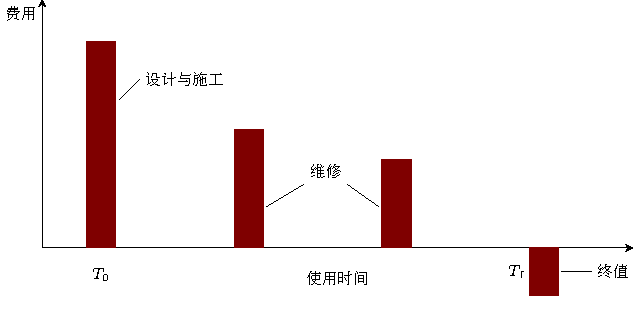
\includegraphics{cash-flow.pdf}
  % \caption{Cash flow diagram}
  \caption{现金流图}
  \label{fig:cash-flow-diagram}
\end{figure}

% Usually on cash flow diagrams, all resource flows are attributed to either the beginning or the end of the time period in which they actually occur. In cases in which a resource flow is extended over several periods, the expenses are represented as a series of lines. It is important to note that cash flow diagram expenses are shown as lines graphed in the positive domain, while revenues and other returns (e.g., the terminal value of the bridge) are shown as negative values. For simplicity, only Agency costs have been plotted on the example cash flow diagram shown in \cref{fig:cash-flow-diagram}. When other types of costs (e.g., user costs and vulnerability costs) are included, the cash flow diagram serves as a graphic representation of the NPV computation.
通常在现金流图上,所有资源流量都归因于它们实际发生的时间段的开始或结束。在资源流扩展到多个时期的情况下,费用表示为一系列线。值得注意的是,现金流量图费用显示为正域中的线图,而收入和其他回报(例如,桥梁的终值)显示为负值。为简单起见,在\cref{fig:cash-flow-diagram} 中所示的示例现金流图上仅绘制了代理成本。当包括其他类型的成本(例如,用户成本和漏洞成本)时,现金流量图用作\acrlong{npv}计算的图形表示。

% \subsection{Estimating User Costs}
\subsection{估算用户成本}
\label{subsec:estimate-user-costs}
% Work zone user costs are the increased \acrfull{voc}, delay, and crash costs incurred by highway users as a result of construction, maintenance, or rehabilitation work zones. User costs may represent the greatest data challenge for its consideration in \acrlong{lcca}. When calculated, user costs are often so large that they may substantially exceed agency costs, particularly for transportation investments being considered for high traffic areas. Congestion statistics and cost can be obtained from the Annual Urban Mobility Report prepared by the Texas Transportation Institute\cite{schrank2011t}.
\gls*{workzone}用户成本是高速公路用户因建设、维护或修复\gls*{workzone}而增加的\acrfull{voc}、延误和事故成本。用户成本可能代表其在\acrlong*{lcca}中考虑的最大数据挑战。计算时,用户成本通常如此之大,以至于它们可能大大超过代理成本,特别是对于考虑在高交通区域进行的交通投资。拥堵统计数据和成本可以从德克萨斯交通研究所准备的年度城市交通报告中获得 \cite{schrank2011t}。

% The publication Life-Cycle Cost Analysis in Pavement Design, by the FHWA (Walls and Smith 1998), includes a rational step-by-step procedure for determining user costs associated with work zones. Work Zone is defined in the Highway Capacity Manual (TRB 2010) as an area of a highway where maintenance and construction operations impinge on the number of lanes available to traffic or affect the operational characteristics of traffic flowing through the area. In order to analyze work zone user costs, work zone characteristics associated with alternative designs and supporting maintenance and rehabilitation strategies must be defined as part of the development of alternative designs.
\acrshort*{fhwa} 出版的 \bkn*{The publication Life-Cycle Cost Analysis in Pavement Design} \cite{walls1998l} 包括一个合理的分步程序,用于确定与\gls*{workzone}相关的用户成本。\bkn*{Highway Capacity Manual} (TRB 2010) 将\gls*{workzone}定义为公路上的一个区域,在该区域中,维护和施工作业会影响可供交通使用的车道数量或影响流经该区域的交通的运营特征。为了分析\gls*{workzone}用户成本,必须将与备选方案设计相关的\gls*{workzone}特征以及支持维护和修复策略定义为备选方案设计开发的一部分。

% Key work zone characteristics include such factors as work zone length, number and capacity of lanes open, duration of lane closure timing (e.g., hours of the day, days of the week, season of the year, etc.), posted speed, and the availability of, and the physical and traffic characteristics of alternative routes. The strategy for maintaining traffic should include any anticipated restrictions on the contractor’s or maintenance force’s hours of operation or ability to establish lane closures.
关键\gls*{workzone}特征包括\gls*{workzone}长度、开放车道的数量和通行能力、车道关闭时间的持续时间(例如,一天中的几个小时、一周中的几天、一年中的季节等)、公布的速度和备选路线的可用性以及物理和交通特征。维持交通的策略应包括对承包商或维护人员的运营时间或建立车道封闭能力的任何预期限制。

% Specific details in an \acrlong*{lcca} should include:
\acrlong*{lcca} 中的具体细节应包括:
% \begin{enumerate}
%   \item Projected year work zones occur (years 5, 8, 12, etc.);
%   \item Number of days the work zone will be in place (construction period);
%   \item Specific hours of each day, as well as the days of the week the work zone will be in place; and
%   \item Work zone length and posted speed.
% \end{enumerate}
\begin{enumerate}
  \item 预计出现\gls*{workzone}年份(第 5 年、第 8 年、第 12 年等);
  \item \gls*{workzone}将到位的天数(施工期);
  \item 每天\gls*{workzone}到位的小时数,以及\gls*{workzone}出现在一周中的哪几天;
  \item \gls*{workzone}长度和发布速度。
\end{enumerate}

% The duration of a work zone (the overall length of time a facility or portion of a facility is out of service or traffic is restricted) can range from sporadic daily lane closures for maintenance to several months for bridge deck replacements. In many cases, the differential routine maintenance cost between alternatives tends to be insignificant when compared to initial construction and rehabilitation costs. To a great extent, the same is true of user costs resulting from routine maintenance activities. Routine maintenance work zones tend to be relatively infrequent, of short duration, and outside of peak traffic flow periods. As such, attention should focus on user costs associated with major work zones.
\gls*{workzone}的持续时间(设施或设施的一部分停止服务或交通受限的总时间长度)范围可以从零星的每日车道关闭以进行维护到长达几个月的桥面更换。在许多情况下,与初始建设和修复成本相比,备选方案之间的差异性日常维护成本往往微不足道。在很大程度上,日常维护活动产生的用户成本也是如此。例行维护的\gls*{workzone}往往出现得相对不频繁,持续时间较短,并且在交通流量高峰期之外。 因此,应将注意力集中在与主要\gls*{workzone}相关的用户成本上。

% User costs are directly dependent on the effects of the volume and operating characteristics of the traffic on the facility. Each construction, maintenance, and rehabilitation activity generally involves some temporary effect on traffic using the facility, varying from insignificant for minor work zone restrictions on low-volume facilities to highly significant for major lane closures on high-volume facilities.
用户成本直接取决于交通量和运营特征对设施的影响。 每项建设、维护和修复活动通常会对使用设施的交通产生一些临时影响,从对低流量设施的次要\gls*{workzone}限制微不足道到对高流量设施的主要车道关闭非常重要。

% The major traffic characteristics of interest for each year that a work zone will be established include:
每年将建立\gls*{workzone}的主要交通特征包括:
% \begin{enumerate}
%   \item Overall projected average annual daily traffic (AADT) volumes on both the facility and possibly alternate routes;
%   \item Associated 24-hour directional hourly demand distributions; and
%   \item Vehicle classification distribution of the projected traffic streams.
% \end{enumerate}
\begin{enumerate}
  \item 设施和可能的备选路线的总体预计\acrfull{aadt};
  \item 关联的 24 小时定向小时需求分布;
  \item 预计交通流的车辆类型分布。
\end{enumerate}

% On high-volume routes, distinctions between weekday and weekend traffic demand and hourly distributions become important. Further, seasonal AADT traffic distribution also becomes important when work zones are proposed on recreational routes during seasonal peak periods.
在大流量路线上,区分工作日和周末的交通需求以及每小时的分布变得很重要。此外,当在季节性高峰期在休闲路线上提议设立\gls*{workzone}时,季节性\acrlong*{aadt}交通分布也变得很重要。

% Once the individual work zones have been identified, each is evaluated separately. This is the point at which individual user cost components are quantified and converted to dollar cost values. A detailed example of the user cost calculation is given in the 1998 FHWA publication, Life Cycle Cost Analysis in Pavement Design (Walls and Smith 1998).
一旦确定了各个\gls*{workzone},就会对每个\gls*{workzone}进行单独评估。 这是单个用户成本构成被量化并转换为美元成本值的点。 用户成本计算的详细示例在 1998 年 FHWA 出版物 \bkn*{Life Cycle Cost Analysis in Pavement Design} \cite{walls1998l} 中给出。

% As mentioned in \cref{subsubsec:user-costs}, the recent pooled-fund study led by the Oregon DOT (Doolen, et al. 2011) developed a set of decision making tools to evaluate the cost effectiveness of using ABC techniques versus. conventional construction, and incorporated user costs as part of the life-cycle cost analysis comparison. The tools also incorporated an analytical hierarchy process (AHP), which is a technique that aids decision makers in prioritizing multiple criteria, and uses a multi-level hierarchical structure of objectives, criteria and alternatives. It considers both quantitative and qualitative criteria and quantifies the qualitative trade-offs and relationship between criteria using a hierarchy of criteria. This was important for ABC because it quantified various qualitative factors contributing to user costs, such as user delay from a long detour, and could show the economic benefit resulting from reduced construction duration.
正如\cref{subsubsec:user-costs}中提到的,最近由俄勒冈\acrlong*{dot}领导的联合基金研究 \cite{doolen2011a} 开发了一套决策工具来评估使用 \acrshort*{abc} 技术与使用传统施工技术的成本效益比较,并将用户成本作为生命周期成本分析比较的一部分。 这些工具还结合了\acrfull{ahp},这是一种帮助决策者确定多个标准优先级的技术,并使用目标、标准和备选方案的多层次结构。它考虑了定量和定性标准,并使用标准层次结构量化了定性权衡和标准之间的关系。这对 \acrshort*{abc} 很重要,因为它量化了导致用户成本的各种定性因素,例如用户因长途绕行而造成的延误,并且可以显示缩短施工工期带来的经济效益。


% \subsection{Computational Approaches}
\subsection{计算方法}
\label{subsec:computational-approaches}
% The two approaches used in preparing an \acrlong*{lcca} differ dramatically in how they address the variability and uncertainty associated with various input factors, and with the risk associated with the various uncertainties. Often there is some level of possible variability and uncertainty in regard to the values identified for each input parameter. This possible variation can often have significant effects on the \acrlong*{lcca} outcome.
用于准备 \acrlong*{lcca} 的两种方法在处理与各种输入因素相关的可变性和不确定性以及与各种不确定性相关的风险方面存在显着差异。对于为每个输入参数确定的值,通常存在某种程度的可能可变性和不确定性。这种可能的变化通常会对\acrlong*{lcca}结果产生重大影响。

% \subsubsection{Deterministic Approach}
\subsubsection{确定性方法}
% Traditionally in the deterministic approach, input variables are treated as fixed values as if those values were certain. This approach assigns each LCCA input variable with a fixed (base case) value based on statistics and nonlinear regression of actually-occurring data, or professional judgment.
传统上,在确定性方法中输入变量被视为固定值,就好像这些值是确定的一样。 这种方法根据实际发生的数据的统计和非线性回归,或专业判断,为每个\acrlong*{lcca}输入变量分配一个固定的(基本)值。

% This method does not specifically address the degree of variability or uncertainty with input values. In order to incorporate uncertainty about input values into the analysis, a sensitivity analysis can be performed to see the effect of variation on any one parameter. However, the deterministic approach combined with the sensitivity analysis has two drawbacks. First, it can only be applied to input variables one-by-one, while in reality the real question of interest is how the variation in several variables simultaneously can affect the result. Even more importantly, sensitivity analysis alone does not provide any information on the relative likelihood of different outcomes. For example, the sensitivity analysis may suggest that if the initial construction cost is 10\% higher than is assumed in the base case, the corresponding NPV of all costs would be 7\% higher than in the base case. However, it will provide no information on whether this scenario is likely to occur. In order to characterize relative likelihood of various potential outcomes, a stochastic approach should be adopted.
该方法没有具体解决输入值的可变性或不确定性程度。为了将输入值的不确定性纳入分析,可以执行灵敏度分析以查看变化对任何一个参数的影响。然而,确定性方法与敏感性分析相结合有两个缺点。首先,它只能一个一个地应用于输入变量,而实际上真正感兴趣的问题是多个变量同时变化如何影响结果。更重要的是,单独的敏感性分析并不能提供关于不同结果的相对可能性的任何信息。例如,敏感性分析可能表明,如果初始建设成本比基本案例中的假设高 10\%,则所有成本的相应\acrlong*{npv}将比基本案例高 7\%。 但是,它不会提供有关这种情况是否可能发生的信息。为了表征各种潜在结果的相对可能性,应采用随机方法。

% \subsubsection{Stochastic Approach}
\subsubsection{随机方法}
% Stochastic approach (sometimes referred to as probabilistic approach, or risk analysis approach) defines the value of input variables by a frequency (probability) distribution. For a given project alternative, the uncertain input parameters are identified. Then, for each uncertain parameter, a sampling distribution of possible values is developed. Simulation programming randomly draws values from the stochastic description of each input variable and uses these values to compute a forecasted NPV. This sampling process is repeated through thousands of iterations, and through the process, an entire probability distribution of NPVs is generated for the project alternative along with the mean or average NPV for that alternative. The resulting NPV distribution can then be compared with the projected NPVs for alternatives, and the most economical option for implementing the project can be determined for any given risk level.
随机方法(有时称为概率方法或风险分析方法)通过频率(概率)分布定义输入变量的值。 对于给定的项目备选方案,确定了不确定的输入参数。然后,对于每个不确定参数,开发可能值的抽样分布。模拟编程从每个输入变量的随机描述中随机抽取值,并使用这些值来计算预测的\acrlong*{npv}。 通过数千次迭代重复此抽样过程,并通过该过程为项目备选方案生成 NPV 的完整概率分布以及该备选方案的均值或平均\acrlong*{npv}。 然后可以将生成的\acrlong*{npv}分布与备选方案的预计\acrlong*{npv}进行比较,并且可以针对任何给定的风险级别确定实施项目的最经济的选择。

% The concept of risk arises from the uncertainty associated with future events and the inability to know what outcomes will result from particular actions taken today. Risk can be objective or subjective. Subjective risk is a person’s perception of the likelihood of a particular event; this perception of risk may include the ability to avoid the risk and an assessment of the consequences of a particular outcome. Objective risk, on the other hand, incorporates theory, experiments, observation, and other unbiased information. Ultimately, decision makers who are characterized by different degrees of risk tolerance and whose perception of risk is intrinsically subjective make the decisions. . However, the goal of risk analysis is to provide the best-unbiased risk estimates to arm the decision makers with the most accurate representation of objective risk.
风险的概念源于与未来事件相关的不确定性,以及无法知道今天采取的特定行动会产生什么结果。风险可以是客观的或主观的。主观风险是一个人对特定事件发生可能性的看法;这种对风险的认识可能包括避免风险的能力和对特定结果后果的评估。另一方面,客观风险包含理论、实验、观察和其他无偏见的信息。最终,以不同程度的风险承受能力为特征并且对风险的感知在本质上是主观的决策者会做出决策。然而,风险分析的目标是提供最佳无偏风险估计,以最准确地表示客观风险来武装决策者。

% \cref{fig:stochastic-approach-lcca} depicts the stochastic approach as a whole. Stated succinctly, it reflects uncertainty in input factors (e.g., construction and repair costs and the timing of those activities) in the probability distribution of the results. Description of the specific steps involved in stochastic approach follow.
\cref{fig:stochastic-approach-lcca} 描述了整个随机方法。简而言之,它反映了结果概率分布中输入因素(例如建设和维修成本以及这些活动的时间安排)的不确定性。随机方法中涉及的具体步骤的描述如下。

\begin{figure}
  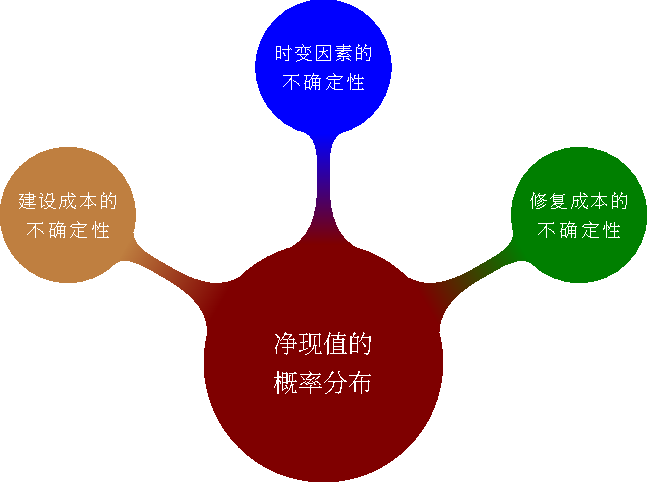
\includegraphics{stochastic-approach.pdf}
  % \caption{Stochastic approach to LCCA}
  \caption{\acrlong*{lcca}的随机方法}
  \label{fig:stochastic-approach-lcca}
\end{figure}

% \emph{Develop Structure and Layout of the Problem}. The first step in conducting risk analysis consists of reducing the problem to its most basic elements and describing it in the form of an analytical model. The models for LCCA problems typically include NPV computation, definition of cost categories, and determination of other functional relationships such as bridge condition curves. Project alternatives are also identified and described. Cash flow diagrams and life-cycle curves are convenient tools to clearly present the project details and the features of alternative implementations.
\emph{制定问题的结构和布局}。 进行风险分析的第一步包括将问题简化为最基本的元素,并以分析模型的形式对其进行描述。\acrlong*{lcca}问题的模型通常包括\acrlong*{npv}计算、成本类别的定义以及其他函数关系(如桥梁状况曲线)的确定。还确定并描述了项目备选方案。 现金流量图和生命周期曲线是清晰呈现项目细节和备选实施方案特征的便捷工具。

% Once the structure of the problem is fully determined, a list of inputs can be developed. An example of input variables for a LCCA project is presented in \cref{tab:lcca-input-variable}. For each of the input variables, the general basis used to determine their values is established, and a subset of input variables for which a stochastic distribution will be used is specified.
一旦问题的结构完全确定,就可以制定输入列表。\acrlong*{lcca}项目的输入变量示例在 \cref{tab:lcca-input-variable} 中给出。 对于每个输入变量,建立用于确定其值的一般基础,并指定将使用随机分布的输入变量子集。

\begin{table}
  % \caption{LCCA Input Variables}
  \caption{\acrlong*{lcca}输入变量}
  \label{tab:lcca-input-variable}
  % \input{tables/lcca-input-variable}
\end{table}

% \emph{Develop Input Data}. The next step in conducting LCCA is developing probability distributions for the uncertain variables identified in the next step. A probability distribution describes the complete range of values that a variable may assume and weighs the likelihood of the occurrence. \cref{fig:example-probability-distributions} illustrates some of the most common probability distributions shown in a histogram format—uniform, triangular, and normal distributions. The horizontal axis provides a range of all possible values that the variable assumes and the vertical axis shows the relative frequency weighting of the occurrence of any particular value. For the distributions on \cref{fig:example-probability-distributions}, the probability of a range of values is equal to the area under the curve, and the total area under the curve is equal to one.
\emph{制定输入数据}。 进行\acrlong*{lcca}的下一步是为下一步确定的不确定变量开发概率分布。概率分布描述了一个变量可能取值的完整范围,并衡量了发生的可能性。\cref{fig:example-probability-distributions} 说明了一些以直方图格式显示的最常见的概率分布——均匀分布、三角分布和正态分布。水平轴提供变量假定的所有可能值的范围,垂直轴显示任何特定值出现的相对频率权重。对于\cref{fig:example-probability-distributions} 上的分布,取值范围的概率等于曲线下的面积,曲线下的总面积等于 1。

% The choice of a particular distribution depends on the type of input and the amount of data available. Triangular distribution (see \cref{fig:example-probability-distributions}) is the most common distribution used to represent various variables using expert elicitation. Expert opinions are used to determine the minimum, the maximum, and the most likely value, and the triangle is constructed using those three points. This method is most appropriate for modeling such input variables as service life, discount rate, work zone delay, etc. Normal distribution is the most common continuous distribution used to represent random variables symmetrically distributed around the mean value. It is usually a good candidate to represent cost-like variables, such as construction cost, maintenance cost, etc. Normal distribution can either be used to represent the information obtained from the expert elicitation or to use data collected from other sources when the amount of data is sufficiently large. On the other hand, when little information about the input variable is available, a uniform distribution might be used as a rough approximation. Uniform distribution assumes that outside of a certain range, the probability of outcomes drops to zero, but within the range we have no information as to which outcomes are more likely, so it is assumed uniform over that range.
特定分布的选择取决于输入类型和可用数据量。三角分布(参见 \cref{fig:example-probability-distributions})是最常见的分布,用于使用专家启发来表示各种变量。专家意见用于确定最小值、最大值和最可能值,并使用这三个点构建三角形。这种方法最适合对诸如使用寿命、折现率、工作区延迟等输入变量建模。正态分布是最常见的连续分布,用于表示围绕均值对称分布的随机变量。它通常是表示类成本变量的一个很好的候选者,例如建设成本、维护成本等。正态分布既可以用来表示从专家启发中获得的信息,也可以用来表示从其他来源收集的数据。数据足够大。另一方面,当有关输入变量的信息很少时,可以使用均匀分布作为粗略的近似值。均匀分布假设在某个范围之外,结果的概率降为零,但在该范围内我们没有关于哪些结果更有可能的信息,因此假设在该范围内是均匀的。

% While normal and uniform distributions are symmetric around their mean values, the triangular distribution can be either symmetric or asymmetric. Other types of common asymmetric distributions are exponential and lognormal. When a large amount of hard data is available, the best distribution can be determined by using statistical techniques to establish goodness of fit for each of them. However, when data availability is limited, triangular distribution can be used as a rough estimate of the distribution shape.
虽然正态分布和均匀分布围绕其平均值对称,但三角分布可以是对称的或不对称的。其他类型的常见不对称分布是指数分布和对数正态分布。当有大量硬数据可用时,可以通过使用统计技术为每个数据建立拟合优度来确定最佳分布。然而,当数据可用性有限时,三角分布可以用作分布形状的粗略估计。

\begin{figure}
  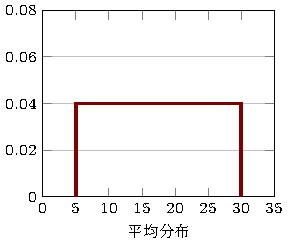
\includegraphics{uniform-distribution.pdf}\hfill
  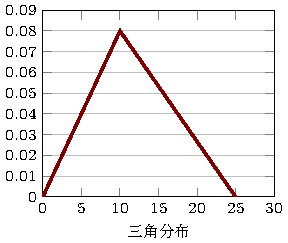
\includegraphics{triangle-distribution.pdf}\hfill
  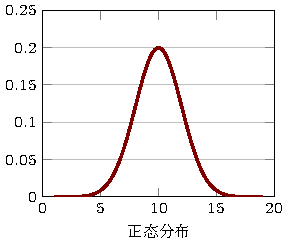
\includegraphics{normal-distribution.pdf}
  % \caption{Example probability distributions}
  \caption{概率分布示例}
  \label{fig:example-probability-distributions}
\end{figure}

\begin{figure}
  % \includegraphics[width=\linewidth]{graphic-file}
  % \caption{Ascending cumulative probability distribution}
  \caption{升序累积概率分布}
  \label{fig:cumulative-probability-distributions}
\end{figure}

% \cref{fig:cumulative-probability-distributions} shows a cumulative probability distribution in ascending order that portrays a cumulative probability of a group of possible events. (Sometimes cumulative distributions are shown in descending order and then the points on the curve show the probability of exceeding a particular value.) For example, there is an 80\% probability that the project cost will not exceed \$4 million. Each probability distribution has a corresponding cumulative distribution. Cumulative distributions present the data in a form that is easy to interpret for the purposes of risk analysis.
\cref{fig:cumulative-probability-distributions} 按升序显示累积概率分布,描述一组可能事件的累积概率。(有时累积分布按降序显示,然后曲线上的点显示超过特定值的概率。)例如,项目成本不超过 400 万美元的概率为 80\%。 每个概率分布都有对应的累积分布。 累积分布以易于为风险分析目的解释的形式呈现数据。

% \emph{Develop Probability Distributions}. When existing data is available, the standard method is to use the data to choose a functional form of a probability distribution that best fits the available data. Many statistical methods and software packages can be used to compare common distribution types with the available data and to determine goodness of fit, in other words, to indicate how well a particular probability distribution fits the data.
\emph{开发概率分布}。当现有数据可用时,标准方法是使用数据选择最适合可用数据的概率分布的函数形式。许多统计方法和软件包可用于将常见分布类型与可用数据进行比较并确定拟合优度,换句话说,表明特定概率分布与数据的拟合程度。

% However, when sufficient relevant data is not readily available, group interviews are often used to develop probabilities of uncertain variables. Expert panels are convened to establish the boundaries and general shape of input distributions. The process of eliciting information from experts may include group meetings, individual interviews, and formal surveys and questionnaires. The goal of expert elicitation is to establish the general shape of input distribution, and to determine if there are any interdependencies among input variables. The process of expert elicitation is shown on \cref{fig:expert-opinion}.
然而,当没有足够的相关数据时,通常会使用小组访谈来确定不确定变量的概率。召集专家小组确定输入分布的边界和一般形状。从专家那里获取信息的过程可能包括小组会议、个人访谈以及正式调查和问卷调查。专家启发的目标是建立输入分布的一般形状,并确定输入变量之间是否存在任何相互依赖性。\cref{fig:expert-opinion} 显示了专家启发的过程。

\begin{figure}
  
\includegraphics{expert-opinion.pdf}
  % \caption{Using expert opinion to develop probability distributions}
  \caption{使用专家意见来开发概率分布}
  \label{fig:expert-opinion}
\end{figure}

% \emph{Perform Simulations}. The next step in the LCCA process involving risk analysis is to run a computer simulation of the model in order to obtain results. A process of using random numbers to sample from a probability distribution is known as Monte Carlo sampling. In the Monte Carlo simulation process, a series of random numbers are generated by the computer along the cumulative probability scale of input distribution (see \cref{fig:cumulative-probability-distributions}). Values corresponding to each random number are sampled along the x-scale. The sampled value for one input is then combined with sampled values for all other inputs to compute the single result. This process is repeated hundreds or thousands of times to generate a cumulative distribution of the outcomes. The stopping rule involves either a prespecified number of iterations or a convergence rule, in other words, a situation in which additional iterations do not significantly affect the distribution of the results.
\emph{执行模拟}。涉及风险分析的\acrlong*{lcca}过程的下一步是运行模型的计算机模拟以获得结果。使用随机数从概率分布中抽样的过程称为蒙特卡洛抽样。在蒙特卡洛模拟过程中,计算机沿着输入分布的累积概率尺度生成一系列随机数(参见 \cref{fig:cumulative-probability-distributions})。对应于每个随机数的值沿 x 尺度采样。 然后将一个输入的采样值与所有其他输入的采样值组合以计算单个结果。此过程重复数百或数千次以生成结果的累积分布。停止规则涉及预先指定的迭代次数或收敛规则,换句话说,额外的迭代不会显着影响结果分布的情况。

% Monte Carlo simulations require a large number of iterations to assure that values with low probabilities are sufficiently sampled and represented in the results. This is especially important when the input distributions are highly unsymmetric. When the number of iterations is insufficient, the low probability outcomes may be underepresented and not adequately accounted for in simulations. This is especially significant when a lowprobability outcome can have a particularly strong effect on the results. In order to avoid such problems, different sampling methods can be employed. For example, Latin Hypercube sampling uses special techniques to generate samples from all probability ranges with a relatively low total number of iterations.
蒙特卡洛模拟需要大量迭代以确保低概率的值被充分采样并在结果中表示。当输入分布高度不对称时,这一点尤为重要。当迭代次数不足时,低概率结果可能会被低估,并且在模拟中没有得到充分考虑。当低概率结果可能对结果产生特别强烈的影响时,这一点尤其重要。为了避免此类问题,可以采用不同的采样方法。例如,拉丁超立方抽样使用特殊技术以相对较少的总迭代次数从所有概率范围内生成样本。

% \emph{Interpret Results}. If the analysis uses the traditional deterministic approach, the only data available to decisionmakers would be the means of the output distributions for the alternatives investigated. Based on the comparisons of the means (50\% probability), the difference between Alternative 1 and Alternative 2 in \cref{fig:risk-profile} is small and may be assumed to be negligible. The risk analysis allows one to evaluate a much more nuanced picture. When interpreting the risk profile on \cref{fig:risk-profile}, it is important to distinguish the upside risk from the downside risk. Downside risk for project costs implies a cost overrun, a chance that the costs will be much higher than anticipated. On the other hand, the upside risk presents an opportunity for low cost, a cost underrun. From \cref{fig:risk-profile}, we can see that Alternative 1 has greater upside risk than Alternative 2, in other words, it has a better chance that the cost will be very low. At the same time, Alternative 1 is a preferred choice because it reduces the downside risk of cost overruns. Another consideration is to compare the two alternatives at the 80\% cumulative probability level. Alternative 1 is about \$100,000 while Alternative 2 is \$130,000. While the means have a negligable risk difference, Alternative 1 exhibits far less of a financial risk.
\emph{解释结果}。如果分析使用传统的确定性方法,则决策者可用的唯一数据将是所调查备选方案的输出分布均值。根据均值(50\% 概率)的比较,\cref{fig:risk-profile} 中的备选方案 1 和备选方案 2 之间的差异很小,可以假设可以忽略不计。风险分析允许人们评估更细微的画面。在解释\cref{fig:risk-profile} 上的风险概况时,区分上行风险和下行风险很重要。项目成本的下行风险意味着成本超支,即成本远高于预期的可能性。另一方面,上行风险提供了低成本、成本不足的机会。从\cref{fig:risk-profile} 可以看出,备选方案 1 的上行风险高于备选方案 2,换句话说,它更有可能成本非常低。同时,备选方案 1 是首选,因为它降低了成本超支的下行风险。 另一个考虑是在 80\% 的累积概率水平上比较两个备选方案。备选方案 1 约为 \num{100000} 美元,而备选方案 2 约为 \num{130000} 美元。虽然这两种方式的风险差异可以忽略不计,但备选方案 1 的财务风险要小得多。

\begin{figure}
  % \includegraphics[width=\linewidth]{graphic-file}
  % \caption{Cumulative risk profile of NPV for Alternatives 1 and 2.}
  \caption{备选方案 1 和 2 的\acrlong*{npv}累积风险概况}
  \label{fig:risk-profile}
\end{figure}

% As a part of the risk assessment, a sensitivity analysis of simulation results can be performed to identify the key input variables that have the most influence on the output distributions. Typically, this is done by computing the degree of correlation between inputs and outputs: the higher the degree of correlation, the more significant a particular input variable is for determining the results.
作为风险评估的一部分,可以对模拟结果进行敏感性分析,以确定对输出分布影响最大的关键输入变量。通常,这是通过计算输入和输出之间的相关程度来完成的:相关程度越高,特定输入变量对于确定结果的重要性就越大。

% From the perspective of most transportation agencies, the application of stochastic LCCA is relatively new. Stochastic LCCA has become more practical due to the dramatic increases in computer processing capabilities. Simulating and accounting for simultaneous changes in LCCA input parameters can now be accomplished easily and quickly and provides invaluable information for making informed decisions.
从大多数运输机构的角度来看,随机\acrlong*{lcca}的应用相对较新。由于计算机处理能力的急剧提高,随机\acrlong*{lcca}变得更加实用。现在可以轻松快速地模拟和计算\acrlong*{lcca}输入参数的同时变化,并为做出明智的决策提供宝贵的信息。


% \subsection{LCCA Analysis Tools}
\subsection{\texorpdfstring{\acrlong*{lcca}}{全生命周期成本分析}的分析工具}
% \subsubsection{Simplified LCCA Applications}
\subsubsection{简化的\acrlong*{lcca}应用程序}
% Various tools and software are available for determining LCCA. All steps of a simplified deterministic LCCA can be performed using generic spreadsheet software such as Microsoft Excel.
有多种工具和软件可用于确定\acrlong*{lcca}。 可以使用 \Microsoft[\Excel] 等通用电子表格软件执行简化的确定性\acrlong*{lcca}的所有步骤。

% For conducting stochastic or risk based LCCA, there are several commercially-available, microcomputer-based risk and analysis software programs that are either spreadsheet based or work as add-ons to other generic spreadsheet software. These tools incorporate Monte Carlo simulation capabilities for stochastic analyses. Two common applications are presented in \cref{tab:software}.
为了进行随机或基于风险的\acrlong*{lcca},有几种商业上可用的、基于微型计算机的风险和分析软件程序,这些程序要么基于电子表格,要么作为其他通用电子表格软件的附件。这些工具结合了用于随机分析的蒙特卡洛模拟功能。\cref{tab:software} 中介绍了两个常见的应用程序。

\begin{table}
  % \caption{Risk Based LCCA software}
  \caption{基于风险分析的\acrlong*{lcca}软件}
  \label{tab:software}
  \begin{tblr}{
  colspec={l X[l]},
  row{1}={bg=genfg,fg=white,font=\bfseries}
}
软件名称 & 生产商 \\
@Risk & {Palisade Corporation \\ \url{https://www.palisade.com}} \\
Oracle Crystal Ball & {Decisioneering Corporation \\ \url{http://www.decisioneering.com}}\\
\end{tblr}
\end{table}

% In using simple generic spreadsheets, the economic life-cycle analysis model has to be programmed into the spreadsheet, and other considerations such as incorporating user costs also have to be computed separately. However, the user has much more control over the process and how data is used and presented. For simple applications, generic spreadsheet solutions are common and easily applied.
在使用简单的通用电子表格时,必须将经济生命周期分析模型编程到电子表格中,并且还必须单独计算其他考虑因素,例如合并用户成本。但是,用户可以更好地控制流程以及数据的使用和呈现方式。对于简单的应用程序,通用电子表格解决方案很常见且易于应用。


% \subsubsection{Comprehensive LCCA Applications}
\subsubsection{综合的\acrlong*{lcca}应用程序}
% Specialized comprehensive software tools for performing LCCA have recently been developed by federal agencies and are available from governing public websites. The available software tools described are capable of calculating comprehensive life-cycle costs including agency, user, operations and maintenance, disposal, and remaining service life costs. They are also capable of performing both deterministic and stochastic analyses.
联邦机构最近开发了用于执行\acrlong*{lcca}的专门综合软件工具,可从管理公共网站获得。所描述的可用软件工具能够计算综合生命周期成本,包括代理成本、用户成本、运营和维护成本、处置成本以及剩余使用寿命成本。它们还能够执行确定性和随机分析。

% \paragraph*{BridgeLCC Software from the National Institute of Standards and Technology (NIST)}
\paragraph*{\acrfull*{nist}开发的软件 BridgeLCC}
% BridgeLCC 2.0 is comprehensive LCCA software developed by the National Institute of Standards and Technology to help bridge designers determine the cost-effectiveness of alternative bridge designs, construction and repair strategies, and construction materials (Ehlen 2003). The software uses a life-cycle costing methodology based on the ASTM E917 standard practice for life-cycle costing and a cost classification scheme developed by NIST (Ehlen 2003). This software is specifically tailored to highway bridges.
BridgeLCC 2.0 是由美国国家标准与技术研究院开发的综合性\acrlong*{lcca}软件,可帮助桥梁设计师确定备选桥梁设计、施工和维修策略以及建筑材料的成本效益 \cite{ehlen2003b}。 该软件使用基于 ASTM E917 生命周期成本计算标准实践和 NIST 开发的成本分类方案的生命周期成本计算方法 \cite{ehlen2003b}。该软件是专门为公路桥梁量身定做的。

% BridgeLCC 2.0 can segregate costs by bearer (agency, user and third party), by timing (initial construction, operations, maintenance and repair [O, M and R], and Disposal), and by component (deck, superstructure, substructure, other, non-elemental and new technology introduction). The program also includes advanced features such as calculation of user delay and cost, has capabilities for both deterministic and stochastic analyses, and includes sensitivity analysis and risk analysis using Monte Carlo simulation (Ehlen 2003).
BridgeLCC 2.0 可以按承担者(机构、用户和第三方)、时间(初始施工、运营、维护和维修 [O、M 和 R],以及处置)和\gls*{component}(桥面系、上部结构、下部结构、其他)分离成本 , 非要素和新技术介绍)。该程序还包括高级功能,例如用户延迟和成本的计算,具有确定性和随机分析的能力,并包括使用蒙特卡罗模拟的敏感性分析和风险分析 \cite{ehlen2003b}。

% \paragraph*{RealCost Life-Cycle Cost Analysis Software}
\paragraph*{RealCost \acrlong*{lcca}软件}

% RealCost was developed by the FHWA to support the application of LCCA in the pavement project-level decision-making process (FHWA 2004). RealCost automates FHWA’s LCCA methodology as it applies to pavements. Work is being considered to make it applicable to bridges but currently, bridges have not been included in this document.
RealCost 由 \acrshort*{fhwa} 开发,用于支持\acrlong*{lcca}在路面项目级决策过程中的应用 \cite{fhwa2004r}。 RealCost 使 \acrshort*{fhwa} 的\acrlong*{lcca}方法自动化,因为它适用于人行道。 正在考虑使其适用于桥梁的工作,但目前,桥梁尚未包含在本文件中。

% The software calculates life-cycle values for both agency and user costs associated with construction and rehabilitation. The software can perform both deterministic and stochastic modeling (Monte Carlo Simulation), and can also include user costs. Outputs are provided in tabular and graphic format.
该软件计算与建设和修复相关的机构和用户成本的生命周期价值。该软件可以执行确定性和随机性建模(蒙特卡罗模拟),还可以包括用户成本。输出以表格和图形格式提供。

% RealCost is an add-in for Microsoft Excel providing a graphical user interface that facilitates the creation an Excel Workbook containing the input data and results of the life-cycle cost analysis. RealCost can only evaluate two alternatives at a time.
RealCost 是 \Microsoft[\Excel] 的一个插件,它提供了一个图形用户界面,有助于创建一个包含\acrlong*{lcca}的输入数据和结果的 \Excel\ 工作簿。 RealCost 一次只能评估两个备选方案。
